\documentclass{article}
\usepackage{tikz-feynman}

\title{Useful Feynmans}

\begin{document}
{
	\section{Wt Decay}
	
	\begin{tikzpicture}
		\begin{feynman}
	
		\vertex (t1) {$t$};
		\vertex [right=of t1] (a);
		\vertex [above right=of a] (t2);
		\vertex [below right=of a] (t3) {$b$};
		\vertex [above right=of t2] (t4) {$\mu^{+}$};
		\vertex [below right=of t2] (t5) {$\nu_{\mu}$};
		
		\diagram* {
			(t1) -- [fermion] (a),
			(a) -- [fermion] (t3),
			(a) -- [boson, edge label=\(W^{+}\)] (t2),
			(t2) -- [fermion] (t4),
			(t2) -- [fermion] (t5),
			};
	
		\end{feynman}
	\end{tikzpicture}
	
	\section{Single Top}
	
	\begin{tikzpicture}
		\begin{feynman}
		
			\vertex (q1) {$q$};
			\vertex [below right=of q1] (a);
			\vertex [below left=of a] (q2) {$\overline{q}$};
			\vertex [right=of a] (b);
			\vertex [below right=of b] (b1) {$\overline{b}$};
			\vertex [above right=of b] (c);
			\vertex [above right=of c] (d);
			\vertex [below right=of c] (b2) {$b$};
			\vertex [above right=of d] (mu) {$\mu^{+}$};
			\vertex [below right=of d] (nu) {$\nu_{\mu}$};
			
			\diagram* {
				(q1) -- [fermion] (a),
				(a) -- [fermion] (q2),
				(a) -- [boson, edge label=\(W^{+}\)] (b),
				(b) -- [fermion] (b1),
				(b) -- [fermion, edge label = \(t\)] (c),
				(c) -- [fermion] (b2),
				(c) -- [boson, edge label = \(W^{+}\)] (d),
				(d) -- [fermion] (mu),
				(d) -- [fermion] (nu),
					};
		\end{feynman}
	\end{tikzpicture}

	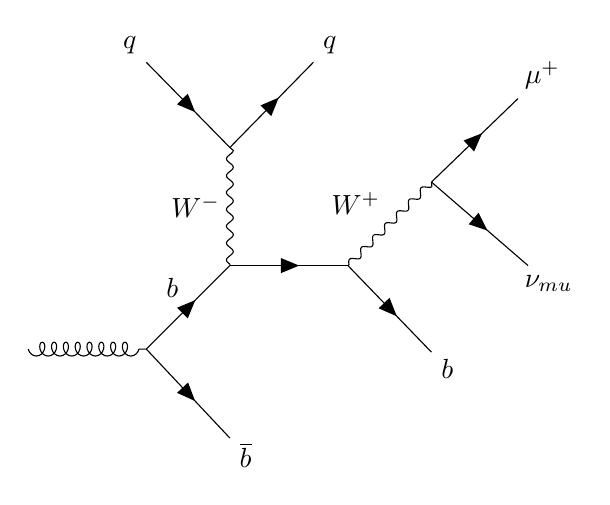
\begin{tikzpicture}
		\begin{feynman}
			\vertex (g1);
			\vertex [right=of g1] (g2);
			\vertex [below right=of g2] (b1) {$\overline{b}$};
			\vertex [above right=of g2] (a);
			\vertex [above=of a] (q2);
			\vertex [above left=of q2] (q1) {$q$};
			\vertex [above right=of q2] (q3) {$q$};
			\vertex [right=of a] (b);
			\vertex [above right=of b] (c);
			\vertex [below right=of b] (b2) {$b$};
			\vertex [above right=of c] (mu) {$\mu^{+}$};
			\vertex [below right=of c] (nu) {$\nu_{mu}$};
			
			\diagram* {
				(g1) -- [gluon] (g2),
				(g2) -- [fermion] (b1),
				(g2) -- [fermion, edge label =$b$] (a),
				(a) -- [boson, edge label = $W^{-}$] (q2),
				(q1) -- [fermion] (q2),
				(q2) -- [fermion] (q3),
				(a) -- [fermion] (b),
				(b) -- [fermion] (b2),
				(b) -- [boson, edge label=$W^{+}$] (c),
				(c) -- [fermion] (mu),
				(c) -- [fermion] (nu),
				};
			
		\end{feynman}
	\end{tikzpicture}

	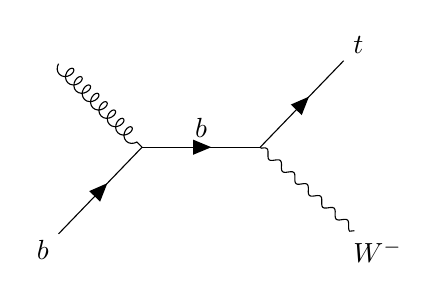
\begin{tikzpicture}
		\begin{feynman}
		
			\vertex (g1);
			\vertex [below right=of g1] (a);
			\vertex [below left=of a] (b1) {$b$};
			\vertex [right=of a] (b);
			\vertex [above right=of b] (t) {$t$};
			\vertex [below right=of b] (w) {$W^{-}$};
			
			\diagram* {
				(g1) -- [gluon] (a),
				(b1) -- [fermion] (a),
				(a) -- [fermion, edge label = $b$] (b),
				(b) -- [fermion] (t),
				(b) -- [boson] (w),
				};
		
		\end{feynman}
	\end{tikzpicture}

	\section{Ttbar}
	
	\begin{tikzpicture}
		\begin{feynman}
			
			\vertex (q1) {$q$};
			\vertex [below right=of a] (a);
			\vertex [below left=of a] (q2) {$\overline{q}$};
			\vertex [right=of a] (b);
			\vertex [above right = of b] (c);
			\vertex [below right = 0.75cm of c] (b1) {$b$};
			\vertex [above right = of c] (d);
			\vertex [above right = of d] (nu1) {$\nu_{\mu}$};
			\vertex [below right = of d] (mu1) {$\mu^{+}$};
			\vertex [below right = of b] (e);
			\vertex [above right = 0.75cm of e] (b2) {$\overline{b}$};
			\vertex [below right = of e] (f);
			\vertex [above right = of f] (mu2) {$\mu^{-}$};
			\vertex [below right = of f] (nu2) {$\nu_{\mu}$};
			
			\diagram* {
				(q1) -- [fermion] (a),
				(a) -- [fermion] (q2),
				(a) -- [boson, edge label = $Z$] (b),
				(b) -- [fermion, edge label = $t$] (c),
				(c) -- [fermion] (b1),
				(c) -- [boson, edge label = $W^{+}$] (d),
				(mu1) -- [fermion] (d),
				(d) -- [fermion] (nu1),
				(e) -- [fermion, edge label'= $\overline{t}$] (b),
				(b2) -- [fermion] (e),
				(e) -- [boson, edge label'=$W^{-}$] (f),
				(f) -- [fermion] (mu2),
				(f) -- [fermion] (nu2),
			};
			
		\end{feynman}
	\end{tikzpicture}

	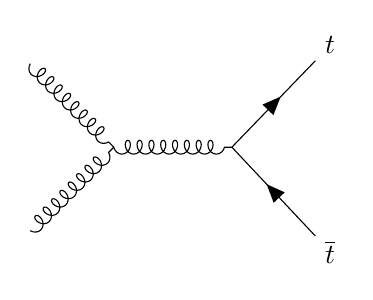
\begin{tikzpicture}
		\begin{feynman}
		
			\vertex (g1);
			\vertex [below right = of g1] (a);
			\vertex [below left = of a] (g2);
			\vertex [right = of a] (b);
			\vertex [above right = of b] (t1) {$t$};
			\vertex [below right = of b] (t2) {$\overline{t}$};
			
			\diagram* {
				(g1) -- [gluon] (a),
				(g2) -- [gluon] (a),
				(a) -- [gluon] (b),
				(b) -- [fermion] (t1),
				(t2) -- [fermion] (b),
			};
		\end{feynman}
	\end{tikzpicture}
	
	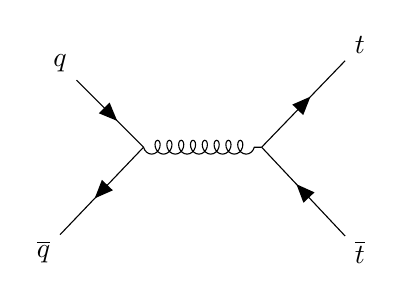
\begin{tikzpicture}
		\begin{feynman}
		
			\vertex (q1) {$q$};
			\vertex [below right = of q1] (a);
			\vertex [below left = of a] (q2) {$\overline{q}$};
			\vertex [right = of a] (b);
			\vertex [above right = of b] (t1) {$t$};
			\vertex [below right = of b] (t2) {$\overline{t}$};
		
			\diagram* {
				(q1) -- [fermion] (a),
				(a) -- [fermion] (q2),
				(a) -- [gluon] (b),
				(b) -- [fermion] (t1),
				(t2) -- [fermion] (b),
				};
				
		\end{feynman}
	\end{tikzpicture}
	
	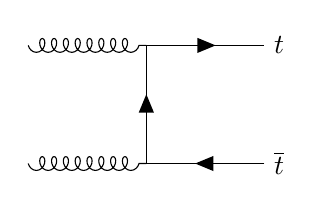
\begin{tikzpicture}
		\begin{feynman}
		
			\vertex (g1);
			\vertex [right = of g1] (a);
			\vertex [right = of a] (t1) {$t$};
			\vertex [below = of a] (b);
			\vertex [left = of b] (g2);
			\vertex [right = of b] (t2) {$\overline{t}$};
		
			\diagram* {				
				(g1) -- [gluon] (a),
				(a) -- [fermion] (t1),
				(b) -- [fermion] (a),
				(g2) -- [gluon] (b),
				(t2) -- [fermion] (b),				
				};
		
		\end{feynman}
	\end{tikzpicture}
	
	\section{Diboson}
	
	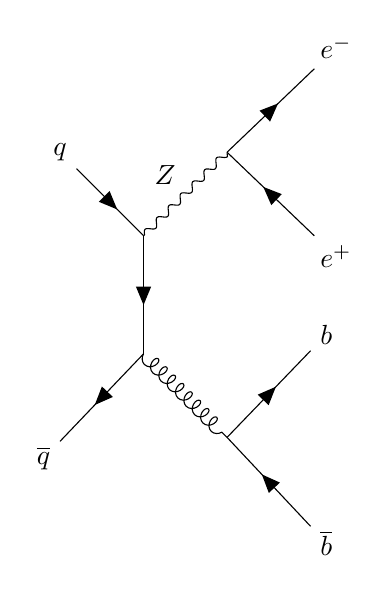
\begin{tikzpicture}
		\begin{feynman}
		
			\vertex (q1) {$q$};
			\vertex [below right = of q1] (a);
			\vertex [below = of a] (b);
			\vertex [below left = of b] (q2) {$\overline{q}$};
			\vertex [above right = of a] (c);
			\vertex [above right = of c] (mu1) {$e^{-}$};
			\vertex [below right = of c] (mu2) {$e^{+}$};
			\vertex [below right = of b] (d);
			\vertex [above right = of d] (b1) {$b$};
			\vertex [below right = of d] (b2) {$\overline{b}$};
			
			\diagram* {
				(q1) -- [fermion] (a),
				(a) -- [fermion] (b),
				(b) -- [fermion] (q2),
				(a) -- [boson, edge label = $Z$] (c),
				(b) -- [gluon] (d),
				(c) -- [fermion] (mu1),
				(mu2) -- [fermion] (c),
				(d) -- [fermion] (b1),
				(b2) -- [fermion] (d),
					};
				
		\end{feynman}
	\end{tikzpicture}
	
	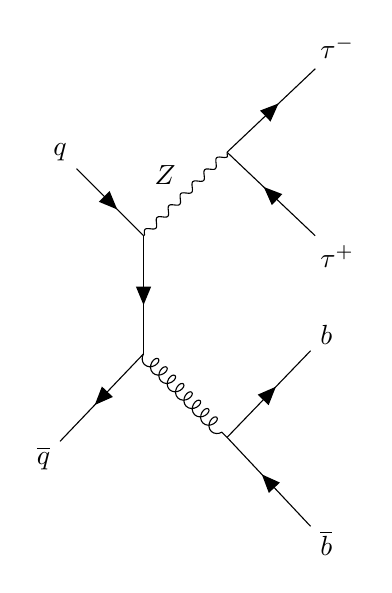
\begin{tikzpicture}
	\begin{feynman}
	
	\vertex (q1) {$q$};
	\vertex [below right = of q1] (a);
	\vertex [below = of a] (b);
	\vertex [below left = of b] (q2) {$\overline{q}$};
	\vertex [above right = of a] (c);
	\vertex [above right = of c] (mu1) {$\tau^{-}$};
	\vertex [below right = of c] (mu2) {$\tau^{+}$};
	\vertex [below right = of b] (d);
	\vertex [above right = of d] (b1) {$b$};
	\vertex [below right = of d] (b2) {$\overline{b}$};
	
	\diagram* {
		(q1) -- [fermion] (a),
		(a) -- [fermion] (b),
		(b) -- [fermion] (q2),
		(a) -- [boson, edge label = $Z$] (c),
		(b) -- [gluon] (d),
		(c) -- [fermion] (mu1),
		(mu2) -- [fermion] (c),
		(d) -- [fermion] (b1),
		(b2) -- [fermion] (d),
	};
	
	\end{feynman}
	\end{tikzpicture}
	
	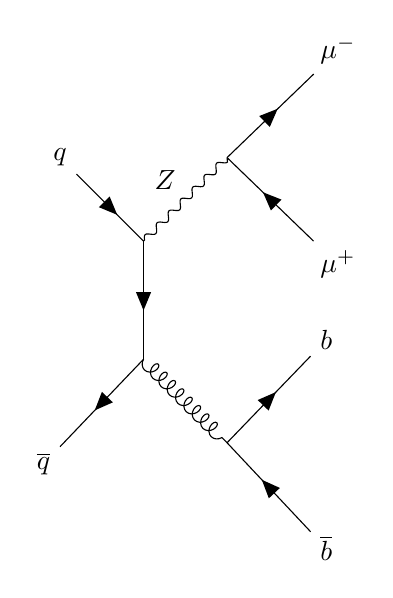
\begin{tikzpicture}
	\begin{feynman}
	
	\vertex (q1) {$q$};
	\vertex [below right = of q1] (a);
	\vertex [below = of a] (b);
	\vertex [below left = of b] (q2) {$\overline{q}$};
	\vertex [above right = of a] (c);
	\vertex [above right = of c] (mu1) {$\mu^{-}$};
	\vertex [below right = of c] (mu2) {$\mu^{+}$};
	\vertex [below right = of b] (d);
	\vertex [above right = of d] (b1) {$b$};
	\vertex [below right = of d] (b2) {$\overline{b}$};
	
	\diagram* {
		(q1) -- [fermion] (a),
		(a) -- [fermion] (b),
		(b) -- [fermion] (q2),
		(a) -- [boson, edge label = $Z$] (c),
		(b) -- [gluon] (d),
		(c) -- [fermion] (mu1),
		(mu2) -- [fermion] (c),
		(d) -- [fermion] (b1),
		(b2) -- [fermion] (d),
	};
	
	\end{feynman}
	\end{tikzpicture}
	
	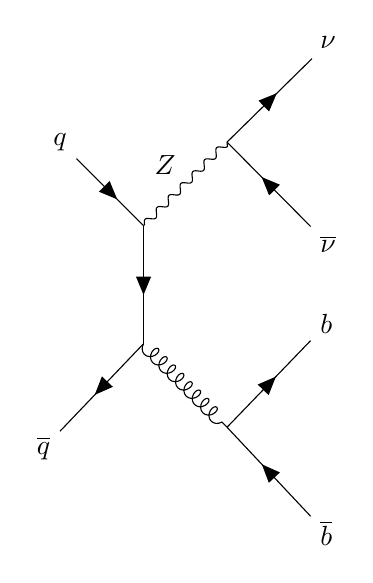
\begin{tikzpicture}
		\begin{feynman}
		
		\vertex (q1) {$q$};
		\vertex [below right = of q1] (a);
		\vertex [below = of a] (b);
		\vertex [below left = of b] (q2) {$\overline{q}$};
		\vertex [above right = of a] (c);
		\vertex [above right = of c] (mu1) {$\nu$};
		\vertex [below right = of c] (mu2) {$\overline{\nu}$};
		\vertex [below right = of b] (d);
		\vertex [above right = of d] (b1) {$b$};
		\vertex [below right = of d] (b2) {$\overline{b}$};
		
		\diagram* {
			(q1) -- [fermion] (a),
			(a) -- [fermion] (b),
			(b) -- [fermion] (q2),
			(a) -- [boson, edge label = $Z$] (c),
			(b) -- [gluon] (d),
			(c) -- [fermion] (mu1),
			(mu2) -- [fermion] (c),
			(d) -- [fermion] (b1),
			(b2) -- [fermion] (d),
		};
		
		\end{feynman}
	\end{tikzpicture}
	
	Important SUSY background as 
	
	\begin{tikzpicture}
		\begin{feynman}
		
		\vertex (b1) {$\tilde{b}$};
		\vertex [right = of b1] (a);
		\vertex [above right = of a] (b2) {$b$};
		\vertex [below right = of a] (chi) {$\chi$};
		
		\diagram* {
			(b1) -- [fermion] (a),
			(a) -- [fermion] (b2),
			(a) -- [fermion] (chi),
			};
		
		\end{feynman}
	\end{tikzpicture}
	
	\section {ZZ4l}
	
	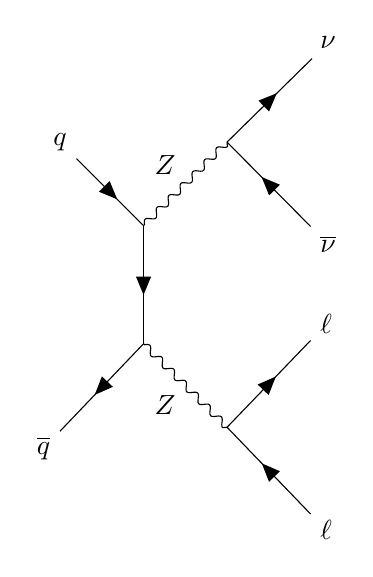
\begin{tikzpicture}
	\begin{feynman}
	
	\vertex (q1) {$q$};
	\vertex [below right = of q1] (a);
	\vertex [below = of a] (b);
	\vertex [below left = of b] (q2) {$\overline{q}$};
	\vertex [above right = of a] (c);
	\vertex [above right = of c] (mu1) {$\nu$};
	\vertex [below right = of c] (mu2) {$\overline{\nu}$};
	\vertex [below right = of b] (d);
	\vertex [above right = of d] (b1) {$\ell$};
	\vertex [below right = of d] (b2) {$\ell$};
	
	\diagram* {
		(q1) -- [fermion] (a),
		(a) -- [fermion] (b),
		(b) -- [fermion] (q2),
		(a) -- [boson, edge label = $Z$] (c),
		(b) -- [boson, edge label'= $Z$] (d),
		(c) -- [fermion] (mu1),
		(mu2) -- [fermion] (c),
		(d) -- [fermion] (b1),
		(b2) -- [fermion] (d),
	};
	
	\end{feynman}
	\end{tikzpicture}
	
}
\end{document}